\documentclass[12pt,a4paper]{article}
\usepackage[utf8]{inputenc}
\usepackage[english]{babel}
\usepackage{amsmath}
\usepackage{amsfonts}
\usepackage{amssymb}
\usepackage{wrapfig}
\usepackage{mathtools}
\usepackage[makeroom]{cancel}
\usepackage{physics}
\usepackage{graphicx}
\usepackage{cancel}
\usepackage[left=3cm,right=3cm,top=2cm,bottom=2cm]{geometry}
\usepackage{physics}
\usepackage{multicol}
\usepackage{caption}
\usepackage{subcaption}
\usepackage{braket} %\braket{a|b|c..}

%main sets:
\newcommand{\Z}{\mathbb{Z}}
\newcommand{\Q}{\mathbb{Q}}
\newcommand{\R}{\mathbb{R}}
\newcommand{\C}{\mathbb{C}}

%math shortcuts
\newcommand{\p}{\partial}
\newcommand{\w}{\omega}
\newcommand{\tf}{\text{TF}}

\DeclarePairedDelimiter{\ceil}{\lceil}{\rceil}



\author{Alessandro Pacco and Marco Biroli}
\title{Report for the seminar:\\Bernard Plaçais, A small tour in graphene flatland}
\begin{document} 
\maketitle


This seminar was held by Mr. Bernard Plaçais on the 14-th of January at ENS.\\

Professor Plaçais is a researcher at the Laboratoire de Physique of the Ecole Nomale Superieure, and his main interests are experimental condensed matter physics and quantum physics. Among his research topics one regards transport in graphene. In particular, during the seminar he brefly introduced us to graphene and to the main uses and technologies for which it is being used and for which it might be used in the future. \\

\begin{figure}[h]
\caption{picture representing an idealized representation of graphene}
\centering
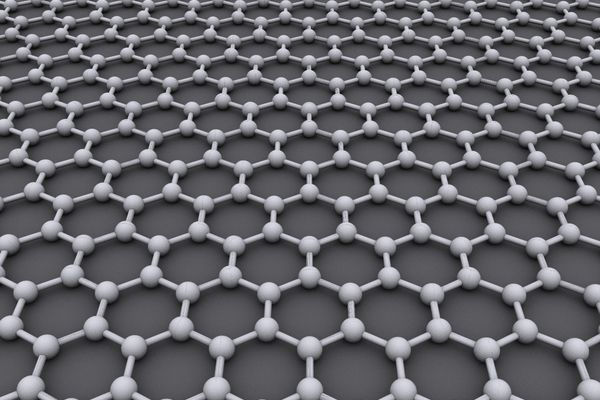
\includegraphics[width=0.5\textwidth]{graphene}
\end{figure}
Graphene is an allotrope of carbon and it consists of a two dimensional hexagonal lattice in which each atom represents a vertex.
Research in single layer graphene physics has started rather recently: before Van der Waals solids were already widely known, however the revolution in graphene was the ability to extract a single layer of graphene. \\
After a brief introduction of what graphene is and the main theorems used in condensed matter, such as Bloch's theorem i.e:
\begin{align*}
\text{In a periodic } &\text{potential the wavefunction takes the following form: } \psi(\vec{r}) = e^{i \vec{k} \cdot \vec{r}} u (\vec{r}) \\ 
&\text{ where } u \text{ has the same periodicity as the potential.}
\end{align*}
We were then introduced to the main applications of graphene. In particular Mr. Placais presented numerous devices that are based on graphene so as to give us an idea of the usefulness of this field of research.
\begin{itemize}
\item The DF-optics dioptre: You tune two different densities of graphene and then you will play with electron waves in graphene.
\item The plasmonic cavity, which is very good for radar applications. Furthermore the advantage of graphene is that it is very cost efficient, and enables to achieve the same frequencies of 20GHz as normal radars.
%  Radars work at typically 20GHz (in mobile phone is about 6GHz), in cars is 70GHz. This is very cost efficient. It's not about beign faster, it's low tech.
\end{itemize}
The magic of graphene is that it has extremely high mobility: when an electron enters graphene it almost doesn't feel that there is a lattice since it will not undergo many collisions. A key feature that confirms this is that the mean free path in graphene scales linearly with the device dimensions. This means that the electrons have little to no knowledge of the lattice background. Another aspect that makes graphene so important and useful for real world applications is that at room temperature the mobility is still very high. For example it would be much more efficient than the materials currently used in our mobile devices. This comes from many factors among which the phonon-cavity coupling. Graphene also has one of the smallest phonon resisitivity out of all current materials, it behaves like a quantum fluid at room temperature.\\
Another important addition to the features and applications of graphene that Mr. Placais presented is that we can do optics with it. An example of which is Dirac electorn optics. The reason why we can use graphene for electron optics is that it is an extremely "clean" material which is something that the presenter insisted on numerous times. For example we can create corner reflectors of Dirac electrons. We also talked about collective modes of the Dirac gas, that is, Dirac plasmons, and we talked about the hydrodynamic phase of the Dirac fluids and the Landau quasiparticle approximation. An important application of graphene to optics is the Zener-Klen graphene transistor, that manages to achieve very high currents. \\\\
Hot electrons in graphene give birth to a particular phenomenon: the Johnson-noise thermometry. Indeed, Professor Bernard Plaçais explained to us that noise can be considered as a signal. If you take a resistor for example, the thermal noise reflects the fact that the electrons have thermal agitation, which in turn makes of it a good thermometer: if you measure the noise you measure the temperature, i.e. thermal agitation of the electrons. Therefore we can measure the temperature of devices by measuring the noise in the transistor. \\
Finally, Professor Plaçais talked about recent improvements in this field. For example a recent revolution consists in the fact that by putting two graphene lattices on top of each other, rotate them and then look at them from above something spectacular happens. The patterns so built are known as moiré patterns or moiré lattices. When doing this with graphene recent studies were able to study new phases of matter such as superfluids and observe the localization/delocalization transition of light (shown by a collaboration lead by the ICFO group: https://www.nature.com/articles/s41586-019-1851-6). \\
In conclusion, graphene is an extremely interesting material due to one key aspect. Since it is an extremely "clean" material that does not affect the electrons travelling through it graphene can be used as a test bench in order to build and observe all type of electronic behavior. Secondly this also allows to build microscopical circuits that have little to no resistivity for practical applications and as an added bonus this can be done in the basement lab of a university since it does not involve any heavy machinery. 







\end{document}
